\usetikzlibrary{arrows.meta,calc}
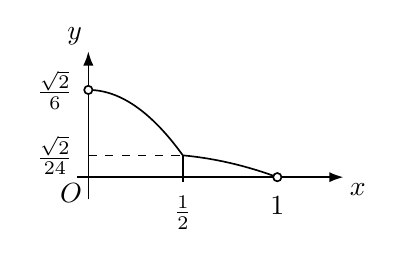
\begin{tikzpicture}[x=2.4cm,y=4.7cm,line width=.6pt,>={Latex[length=1.8mm,width=1.3mm]}]
\def\Vzero{0.235702260396}
\def\Vhalf{0.058925565099}
\coordinate (O) at (0,0);
\coordinate (Y0) at (0,\Vzero);
\coordinate (M) at (0.5,\Vhalf);
\coordinate (X1) at (1,0);
\draw[->] (-0.06,0)--(1.35,0) node[anchor=north west,inner sep=0pt,xshift=2pt,yshift=-2pt] {$x$};
\draw[->] (0,-0.06)--(0,0.34) node[anchor=south east,inner sep=0pt,xshift=-2pt,yshift=2pt] {$y$};
\draw[domain=0:0.5,samples=81] plot (\x,{\Vzero-(\Vzero-\Vhalf)*(\x/0.5)*(\x/0.5)});
\draw[domain=0.5:1,samples=81] plot (\x,{\Vhalf*(1-(\x-0.5)/0.5)*(1+0.6*(\x-0.5)/0.5)});
\draw[dashed] (0,\Vhalf)--(M);
\draw (M)--(0.5,-0.012);
\draw[fill=white] (Y0) circle[radius=1.5pt];
\draw[fill=white] (X1) circle[radius=1.5pt];
\node[left=2pt] at (0,\Vzero) {$\frac{\sqrt2}{6}$};
\node[left=2pt] at (0,\Vhalf) {$\frac{\sqrt2}{24}$};
\node[anchor=north] at (0.5,-0.025) {$\frac12$};
\node[anchor=north] at (1,-0.025) {$1$};
\node[anchor=north east,inner sep=0pt,xshift=-2pt,yshift=-2pt] at (0,0) {$O$};
\end{tikzpicture}
